\chapter{Radio Frequency Interference (RFI) and Site Testing}

\section{Overview}

One of the challenges of radio astronomy is locating sites that meet the environmental requirements of a particular set of observations. Potential sites must be assessed for their viability prior to observation at those sites. I am going to focus here on a specific subset of requirements that are particularly significant for \cm observations. 

First, does the site have any nearby man-made sources of regular radio frequency interference (RFI) in the frequency band of the observations. Evaluation of this requirement can be done using a simple broadband antenna and spectrum analyzer on site at multiple locations. Deployment of an identical system at multiple sites is key in doing comparisons between them. 

Second, are there sources of intermittent or highly time-variable RFI visible from the site. This can be more difficult to evaluate as it requires a long period of data collection. In cases where time-variable RFI is expected to play a significant role in the data collection, semi-permanent systems may need to be installed to track the RFI environment over time. 

Third, is the site logistically accessible for the type of equipment needed for a set of observations. Some important considerations include the availability of power, transport into/out of the location, housing and other observer requirements and site access permissions (such as permits). Assessment of these considerations often requires an in-person visit and careful documentation. 

Fourth, are there atmospheric effects that must be considered in assessing the viability of a site (eg meteor scatter, thickness of ionosphere, inclement weather). Tracking data may be available from external sources such weather surveys, but it is often limited to broad trends instead of local details. 

In the following sections, I am going to evaluate both existing telescope sites and new sites based upon the requirements listed above. I will set a baseline using Pittsburgh, Pennsylvania; which as a major metropolitan area is not expected to be a suitable radio astronomy site. I will then look at several existing radio telescope sites and examine their strengths and weaknesses. Finally, I will report on several new radio sites, comparing them to the existing sites to demonstrate viability. 

\section{Existing Site Evaluations}

\begin{figure}[htb]
\begin{center}
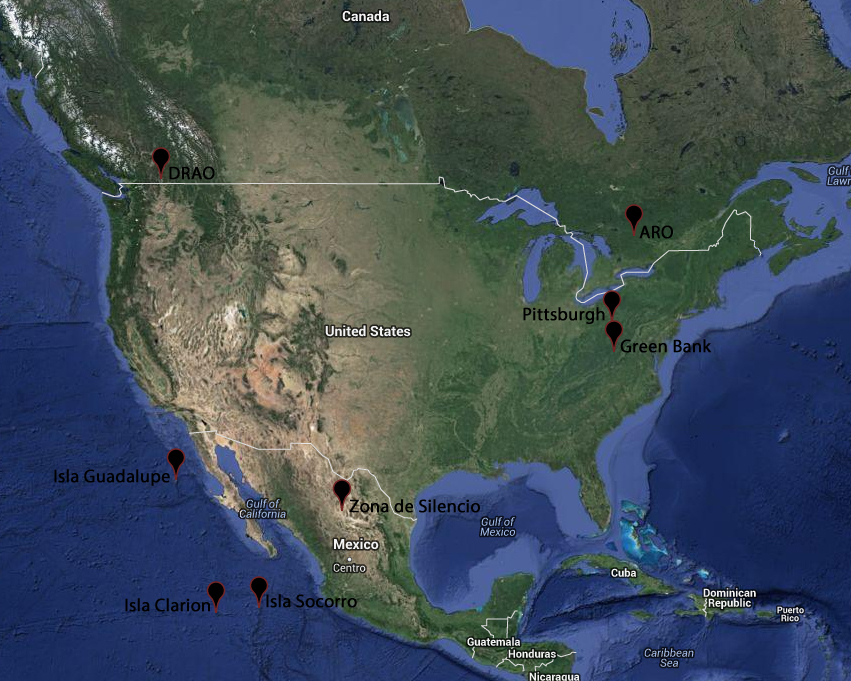
\includegraphics[width=0.95\textwidth]{large_scale_site_map.jpg}
\caption{Map of evaluated sites in North America.}
\label{Fig:site_map}
\end{center}
\end{figure}

One major element of site evaluations was a measurement of the RFI over a wide frequency band at each site. This was measured using a kit composed of a broadband antenna, amplifiers, and a portable spectrum analyzer for data collection. 

By using the same kit at all the sites, the systematic noise contribution to the signal is the same in all datasets. The kit is also highly portable, packing up into a small suitcase and poster tube for easy transport. 

\textcolor{red}{Add in photos of system both in suitcases and assembled on the lawn.}

\subsection{Carnegie Mellon University Pittsburgh, PA, USA}

Carnegie Mellon University is located in the city of Pittsburgh, home to several such universities and possessing a population of over 300,000. As should be expect, the radio environment in Pittsburgh is full of RFI, with signals of such magnitude that they overload test equipment. Figure \ref{Fig:pghrfi} shows the RFI environment in Pittsburgh as measured with my site testing kit. In order to not overload the spectrum analyzer with the high RFI levels at some frequencies, it was necessary to remove one stage of amplification from the system. 

\begin{figure}[htb]
\begin{center}
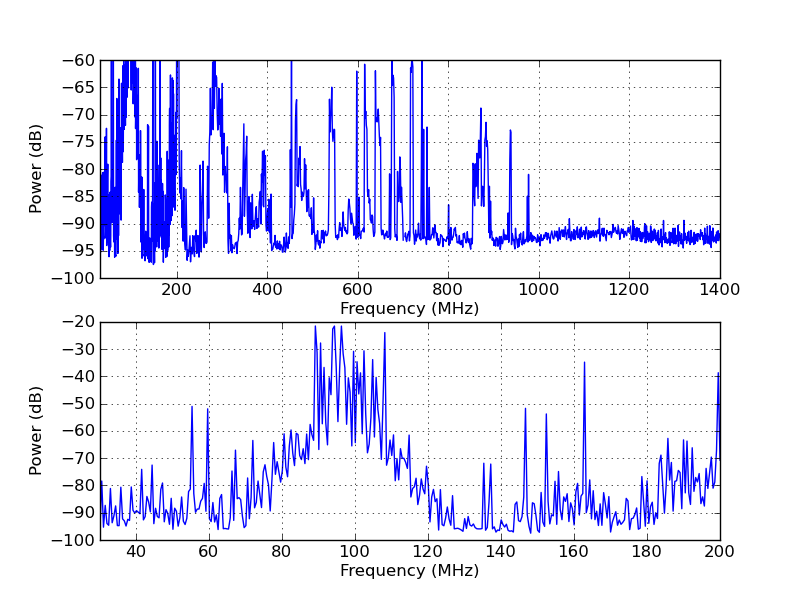
\includegraphics[width=0.95\textwidth]{Pittsburgh_test.png}
\caption{RFI measurement in Pittsburgh, PA.}
\label{Fig:pghrfi}
\end{center}
\end{figure}

\subsection{National Radio Astronomy Observatory (NRAO) Green Bank, WV, USA}

\begin{figure}[htb]
\begin{center}
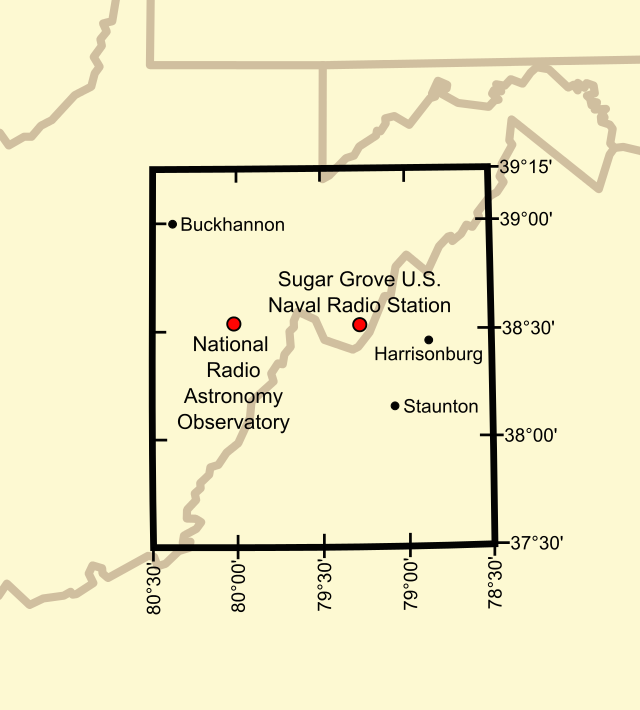
\includegraphics[width=0.8\textwidth]{National_Radio_Quiet_Zone.png}
\caption{Extent of the US National Radio Quiet Zone around the Green Bank Site.}
\label{Fig:nrqz}
\end{center}
\end{figure}

The National Radio Astronomy Observatory (NRAO) is a research center funded by the United States National Science Foundation (NSF). It maintains several telesopes in radio quiet locations. One of these locations is in Green Bank, West Virginia inside the United States National Radio Quiet Zone in Virginia and West Virginia (see Figure \ref{Fig:nrqz}). Within this zone radio broadcasts at all frequencies are extremely limited, allowing for a relatively quiet RFI environment.

The size of the radio quiet zone (about 34,000 $km^2$) is sufficient for the higher \cm frequency range. However, as you go to lower frequencies the size of the zone needed for sufficient shielding becomes larger. This means that the site becomes less ideal for observations as you go to frequencies below 600 MHz (see Figure \ref{Fig:gbtrfi}). The FM band is still significantly contaminated at this site. 

\begin{figure}[htb]
\begin{center}
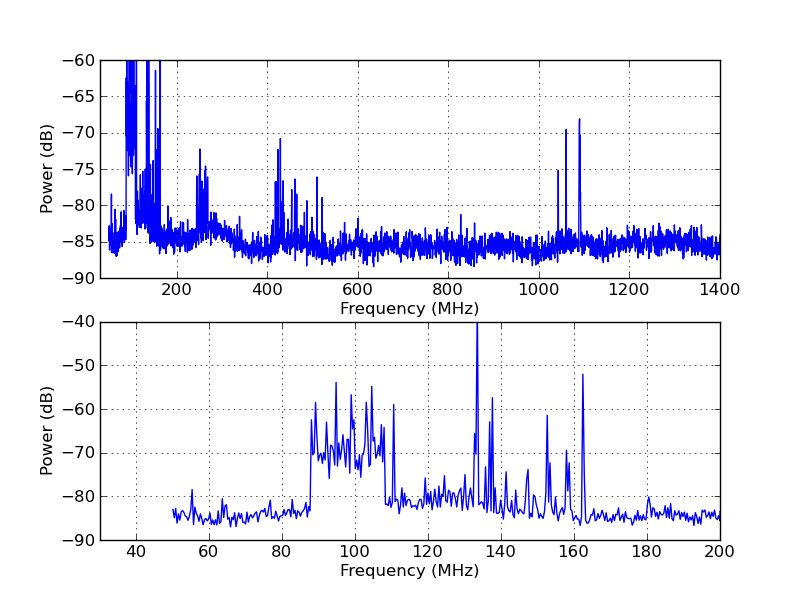
\includegraphics[width=0.95\textwidth]{GBT_subtract.png}
\caption{RFI measurement at the NRAO Green Bank site. }
\label{Fig:gbtrfi}
\end{center}
\end{figure}

\subsection{Dominion Radio Astrophysical Observatory (DRAO) Penticton, BC, Canada}

The Dominion Radio Astrophysical Observatory (DRAO) is a Canadian radio astronomy site located near Penticton, British Columbia in the south-central part of the province. It has a number of radio telescopes on site, including the Canadian Hydrogen Intensity Mapping Experiment (CHIME) system. Like the NRAO Green Bank site, the isolation is insufficient for the lower frequencies. There is significant RFI contamination for most frequencies below 500 MHz at this site (see Figure \ref{Fig:draorfi}). 

\begin{figure}[htb]
\begin{center}
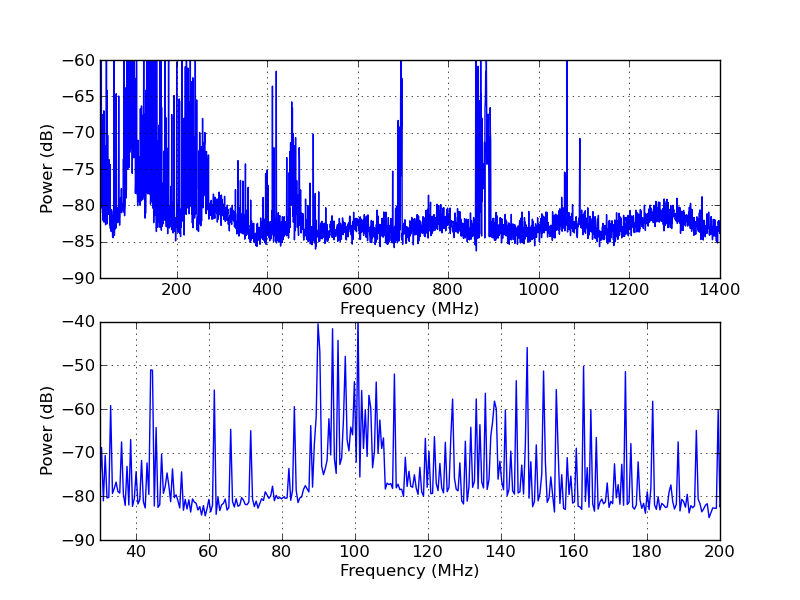
\includegraphics[width=0.95\textwidth]{DRAO_subtract.png}
\caption{RFI measurement at the DRAO Penticton site. }
\label{Fig:draorfi}
\end{center}
\end{figure}


\subsection{Algonquin Radio Observatory (ARO) Algonquin, Ontario, Canada}

The Algonquin Radio Observatory (ARO) is a single instrument Canadian radio astronomy site locaed in the center of Algonquin Provincial Park in Ontario. Accessible only by logging roads, this is a fairly remote site with excellent radio quiet properties. However, Algonquin is still relatively close (about 200-250 km) to the major Canadian metropolitan areas of Toronto and Ottawa. This means that although the rest of the spectrum is quite clean, there is still significant RFI below 300 MHz (see Figure \ref{Fig:arorfi}). 

\begin{figure}[htb]
\begin{center}
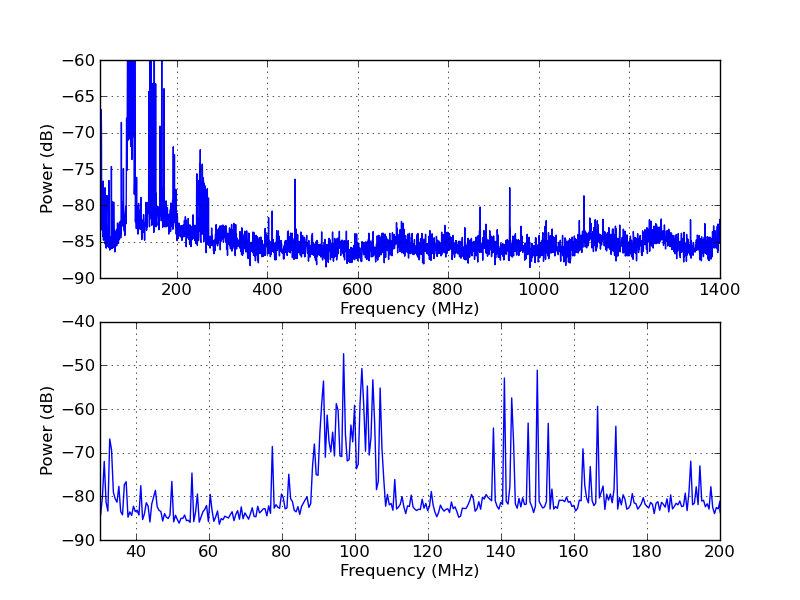
\includegraphics[width=0.95\textwidth]{ALG_subtract.png}
\caption{RFI measurement at the ARO Algonquin site.}
\label{Fig:arorfi}
\end{center}
\end{figure}


\section{New Site Evaluations}

Evaluation of these existing radio quiet sites demonstrates a clear need for sites whose RFI environments are clean to lower frequencies. However, locating such sites can be difficult as the distances required begin to grow large. I will report on a couple of potential sites in Mexico that have significant improvement in their low frequency RFI strength compared to the existing sites. 

\subsection{La Zona de Silencio Mapimi, Mexico}

\subsubsection{Logistics and Current Infrastructure}

Only roads in and out of the site are minimally maintained dirt roads (require 4-wheel drive at a minimum).

Ecology camp inside site has some housing, but the power is provided through solar panels.  Additionally, water availability is also extremely low as there is no local water source. 

\subsubsection{Weather}

Northern mexico is quite hot in summer (desert).

\subsubsection{Measurements}

\begin{figure}[htb]
\begin{center}
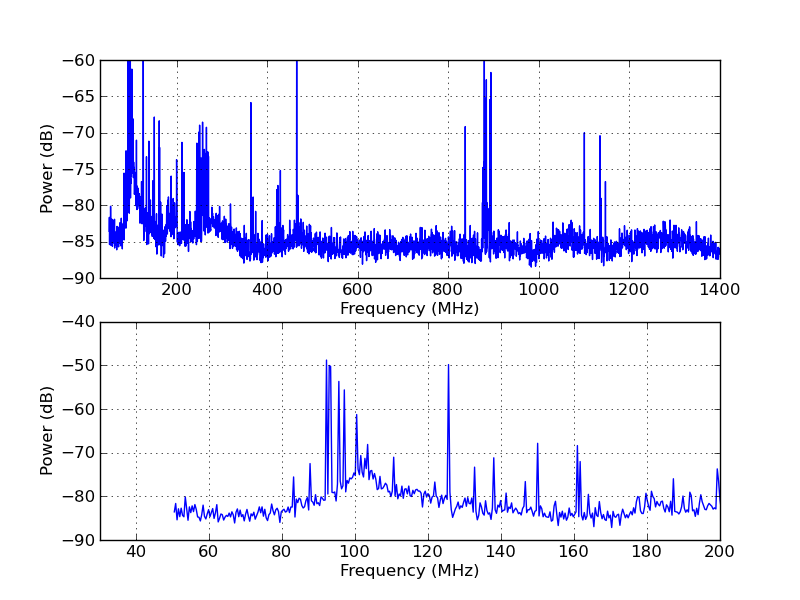
\includegraphics[width=0.95\textwidth]{ZdS_entrance_subtract.png}
\caption{RFI measurement at the entrance to the Zona de Silencio. Note that the FM band is already much cleaner than current sites.}
\label{Fig:zdsentrfi}
\end{center}
\end{figure}

\begin{figure}[htb]
\begin{center}
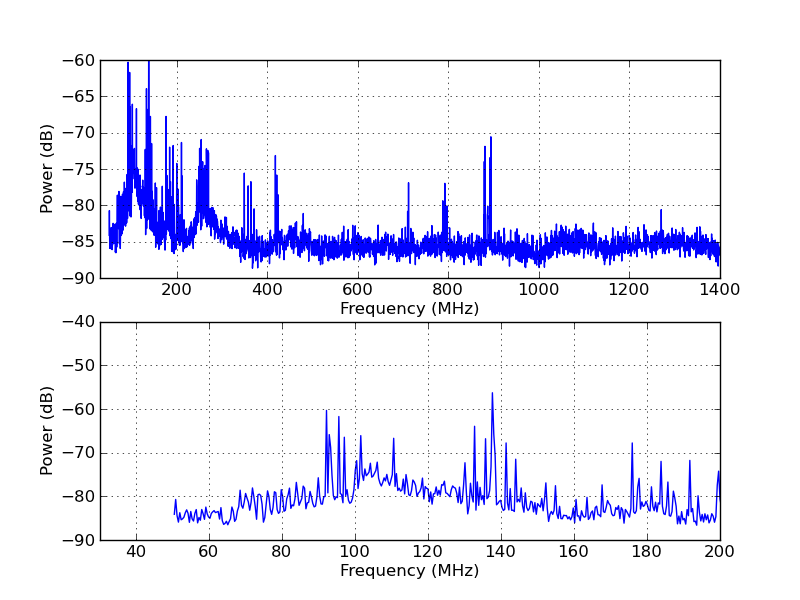
\includegraphics[width=0.95\textwidth]{ZdS_halfway_in_subtract.png}
\caption{RFI measurement part of the way into the Zona de Silencio deployment site. Note that the FM band is still pretty quiet, although it has slightly different structure due to the change of location. }
\label{Fig:zdsmidrfi}
\end{center}
\end{figure}

\begin{figure}[htb]
\begin{center}
\includegraphics[width=0.95\textwidth]{Zds_central_subtract.png}
\caption{RFI measurement at the Zona de Silencio deployment site. At this location there are no strong FM signals, but there is some geneneral low level noise across the band.}
\label{Fig:zdsendrfi}
\end{center}
\end{figure}


\subsection{Isla Guadalupe Baja California, Mexico}

\subsubsection{Logistics and Current Infrastructure}

\subsubsection{Weather}

\subsubsection{Measurements}

\begin{figure}[htb]
\begin{center}
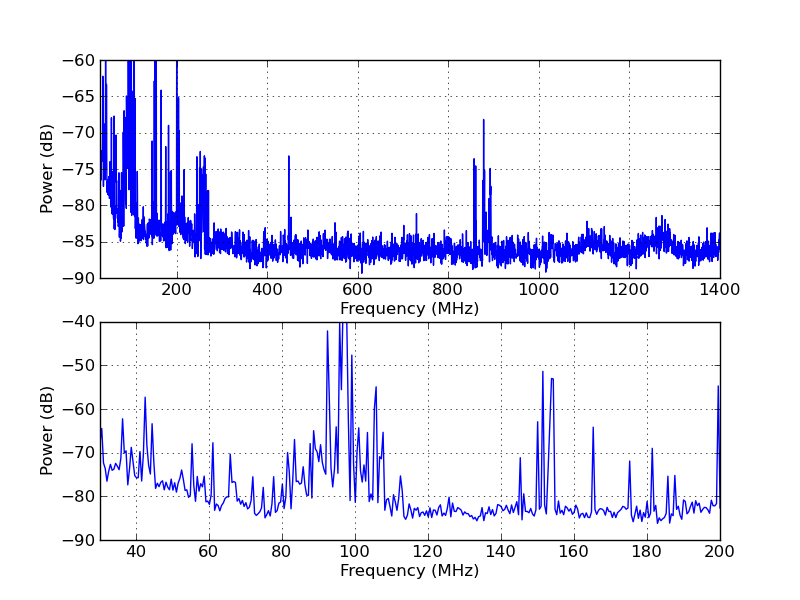
\includegraphics[width=0.95\textwidth]{GI_3__subtract.png}
\caption{RFI measurement at the summit of Guadalupe Island. At this high elevation the FM signals from the mainland are quite strong and there is generally more RFI signals.}
\label{Fig:guadsumrfi}
\end{center}
\end{figure}

\begin{figure}[htb]
\begin{center}
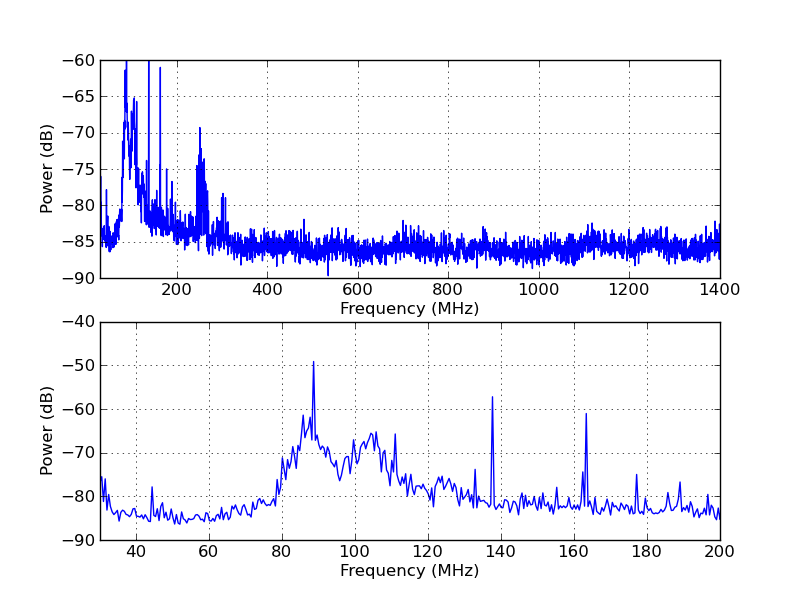
\includegraphics[width=0.95\textwidth]{GI_1__subtract.png}
\caption{RFI measurement near the southern part of Guadalupe Island. This location had a direct line toward the south so picked up some transmissions from FM stations in southern Baja California. }
\label{Fig:guadsouthrfi}
\end{center}
\end{figure}

\begin{figure}[htb]
\begin{center}
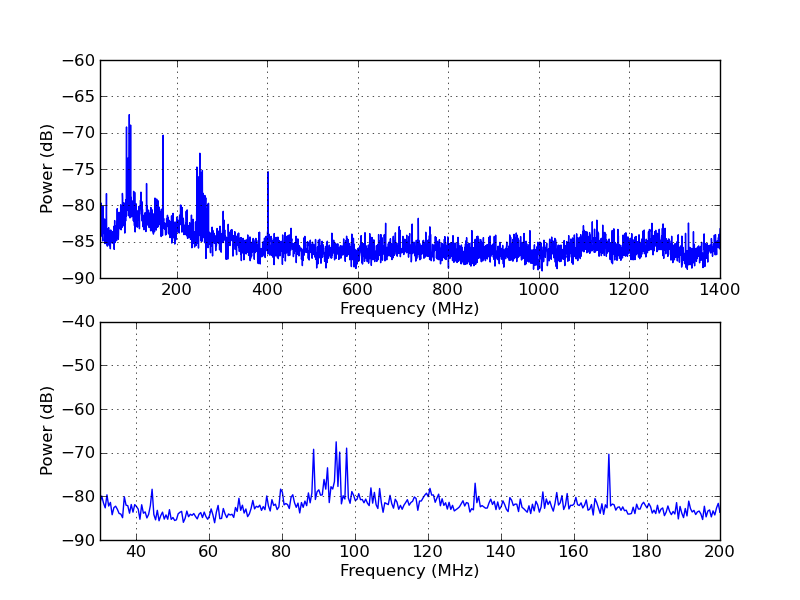
\includegraphics[width=0.95\textwidth]{GI_2__subtract.png}
\caption{RFI measurement from the western side of Guadalupe Island. The peaks of Guadalupe are between this location and the mainland of Baja California, minimizing the RFI environment.}
\label{Fig:guadfishrfi}
\end{center}
\end{figure}


\section{Future Sites}

\subsection{Isla Socorro and Isla Clarion, Mexico}

\subsection{Marion and Gough Islands, South Africa}



